\documentclass[11pt]{article}
\usepackage[margin=1in]{geometry}
\usepackage{fancyhdr}
\usepackage{graphicx}
\usepackage[utf8]{inputenc}
\usepackage[T1]{fontenc}
\usepackage{cite}
\usepackage{xcolor}
\usepackage{listings}
\usepackage{pdfpages}



\pagestyle{fancy}
\fancyhead{}
%\fancyfoot{}
	\fancyhead[L]{Commande BCI}
\fancyhead[R]{Rafael, Mathieu, Heloise}
%\fancyhead[C]{\thepage}

\renewcommand{\contentsname}{\huge{\textbf{Table of Contents}}}

\lstdefinestyle{DOS}
{
    backgroundcolor=\color{black},
    basicstyle=\scriptsize\color{white}\ttfamily
}


\begin{document}

%Title

\begin{titlepage}
\begin{center}

\includegraphics[scale=0.5]{CentraleSupelec.jpeg}\\
\vfill
\line(1,0){400}\\[1mm]
\huge{\textsc{\textbf{Rapport TL SIR Commande de robot par interface cérébrale}}}\\[3mm]
\Large{\textbf{- Rafael ELLER CRUZ, Mathieu, Heloise -}}\\[1mm]
\Large{promo 2018}\\[1mm]
\line(1,0){400}\\[1mm]
%\Large{\textbf{Enseignant Encadrant: VIDAL Micheline}}\\[1mm]
\vfill
%\slshape{Stage chez Smart Prospective, deroulé entre le 19/07/2017 et le 15/09/2017}\\
%\slshape{Incubateur INSEEC 51 Quai de la Seine}\\
\end{center}
\end{titlepage}

%%%Table of contents%%%

\tableofcontents
\thispagestyle{empty}
\cleardoublepage

\pagenumbering{arabic}

%%%Introduction%%%
\setcounter{page}{1}
\section{Introduction}


\cleardoublepage

%%%Étude des signaux%%%

\section{Principes théoriques et définition du problème}


%%%Étude des signaux%%%

\section{Étude des signaux}




\cleardoublepage

%%%Démarche et travaux réalisés%%%

\section{Contrôle du Robot}

 	  
\subsection{}
A footnote \footnote{https://hal.archives-ouvertes.fr/}
%\cite{DBLP:WenG13},

You can see a duck in figure \ref{fig:duck}.

\begin{figure}[!h]
\centering
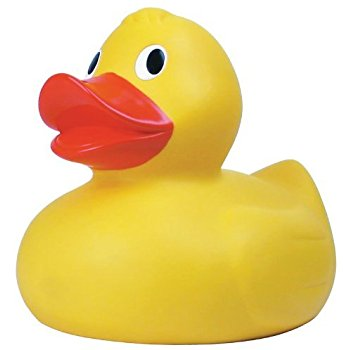
\includegraphics[scale=0.3]{bidon.jpg}
\caption{A duck}
\label{fig:duck}
\end{figure}


\subsubsection{} \label{Deep}

	
\subsubsection{}

\cleardoublepage

%%%Analyse des résultats obtenus%%%

\section{Analyse des résultats}


\subsection{}


\subsection{}

\cleardoublepage

%%%Conclusions et recommandations%%%

\section{Conclusion}

\cleardoublepage

%%%Références bibliographiques%%%

\cleardoublepage

\addcontentsline{toc}{section}{\numberline{}References}
\bibliography{bibl.bib}
\bibliographystyle{ieeetr}

\cleardoublepage

%%%Annexe%%%

\section*{Appendix A:}
\addcontentsline{toc}{section}{\numberline{}Appendix A}

\cleardoublepage

\end{document}
